\begin{figure}
  \centering
  \begin{subfigure}[t]{0.42\textwidth}
    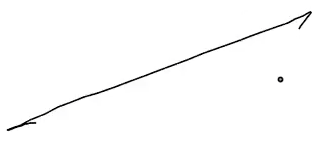
\includegraphics[width=\linewidth]{img/hook-1.png}
    \caption{Raw ink with hooks.}
    \label{fig:hook-1}
  \end{subfigure}
  \hspace{1cm} % spacing, do what you need
  \begin{subfigure}[t]{0.42\textwidth}
    
\includegraphics[width=\linewidth]{img/hook-2.png}
    \caption{Processed ink after hooks removed.}
    \label{fig:hook-2}
  \end{subfigure}
  \caption[Hook removal]{Removing `hooks': accidental short lines at
    the start and end of a stroke.}
  \label{fig:hooks}
\end{figure}
